\chapter{Results \& Discussion}
\section{Results}


Through investigating the walking gait on a large proportion of values, the following data was gathered. A full table of experiments ran can be found in the appendix. 

Figure \ref{froudedistribution} showcases the probability distribution of all values found. The probability distribution showcases a mean  with a Froude number of 0.358, with a variation of 0.283. This is a fairly large variation, which may be due to a large amount of values finding themselves at very low gait values. This show a close adherence to Dynamic Similarity, with a bulk of values finding themselves below gaits of 0.4. In total, out of all of the experiments ran, 72.4\% of values where found to lie below 0.4. 

\begin{figure}[h!]
  \centering
  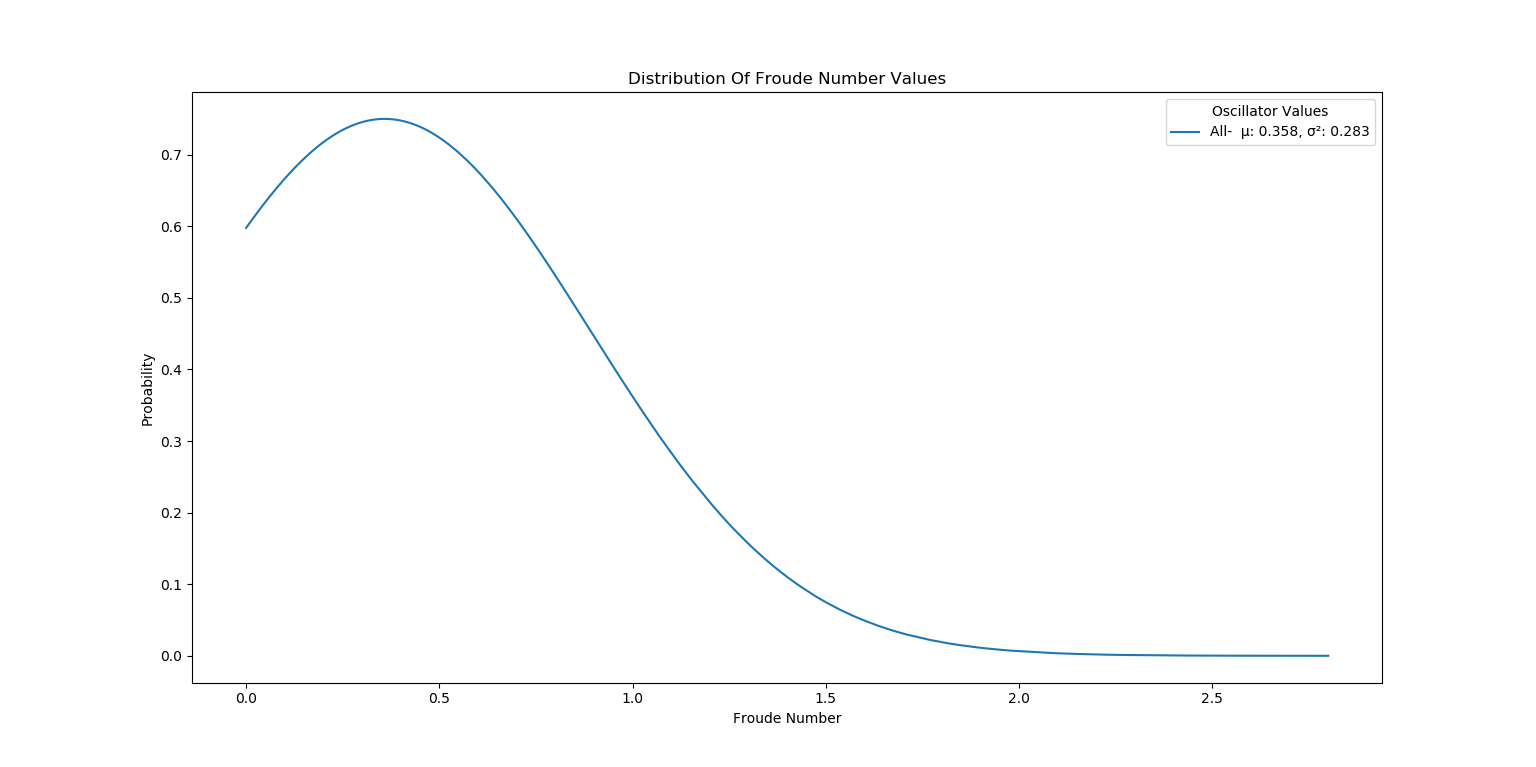
\includegraphics[width=1\textwidth]{USFD_Academic-_Report_LaTeX-Template/figures/froudedistribution.png}
  \caption{Distribution of froude number for all experiments.}
  \label{froudedistribution}
\end{figure}

This distribution does showcase that a large proportion of values are still above 0.4. This does not correlate with the Dynamic Similarity principle, in which Froude numbers of 0.4 are described as the maximum for an animals walking gait, with walking gaits above 0.4 not being seen. An explanation as to why this appears to be due to oscillator time-step, as when filtering the results against oscillator time-step, the distribution seen in figure \ref{froudeosc} are achieved.

\begin{figure}[h!]
    \centering
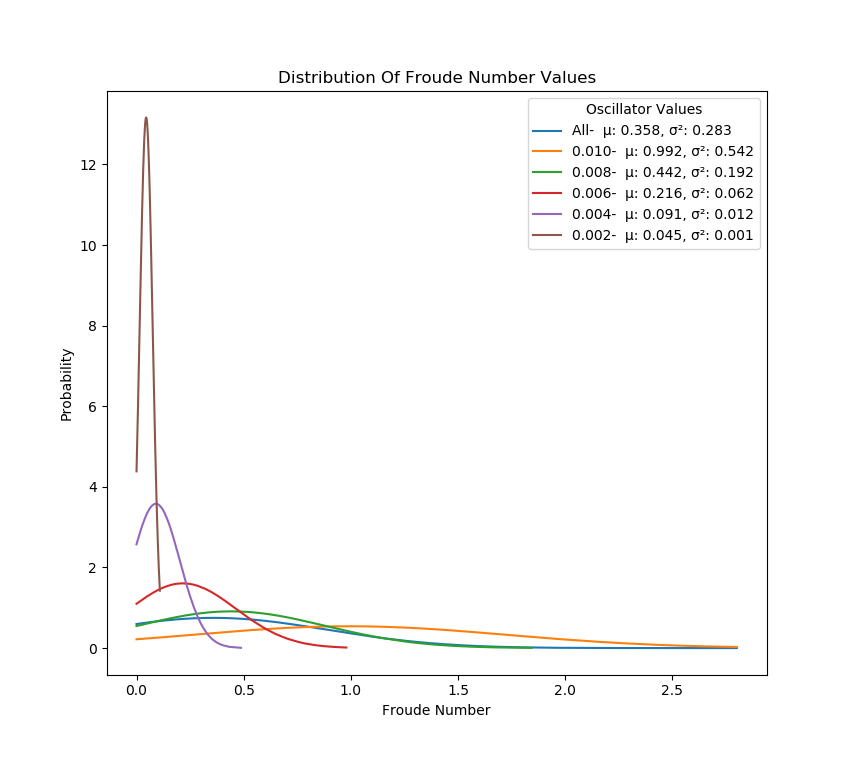
\includegraphics[width=1\textwidth]{USFD_Academic-_Report_LaTeX-Template/figures/froudedistributionoscillator.png}
\caption{Distribution of froude number by oscillation.}
\label{froudedosc}
\end{figure}

This shows that the majority of larger values are found due to larger oscillator time-steps. Above values of 0.008, the mean increases to values far above the range seen in \cite{Alexander1983}. When filtering by oscillator time-steps of 0.006 and below, find that () of results lie within the limits found in Dynamic Similarity. 



% The effects on Froude number when varying forces are far less pronounced, as can be seen through \ref{}
% \begin{figure}[h!]
%     \centering
% \includegraphics[width=1\textwidth]{USFD_Academic-_Report_LaTeX-Template/figures/froudevsforce.png}
% \caption{Distribution of froude number by oscillation.}
% \label{froudefocre}
% \end{figure}

% Although the values reach a peak between 60 and 70, after these values the Froude number reduces. This may be due to a higher variation between values at this point, which suggests that after this point, a large amount of the gaits produced may be unstable

% \section{Cost Of Locomotion}
% Cost of locomotion has been calculated using research shown by \cite{}. Cost of locomotion has been calculated by the following equation.

% Due to the experiment running for a set amoiunt of iterations instead of distance, for this paper, we will be using the cost of locomotion per unit distance travelled. This is in order to allow comparisons between cost of locomotion and velocity, as a robot travelling at a larger velocity may be less efficient than one travelling slower.

% \begin{figure}[h!]
%   \centering
%   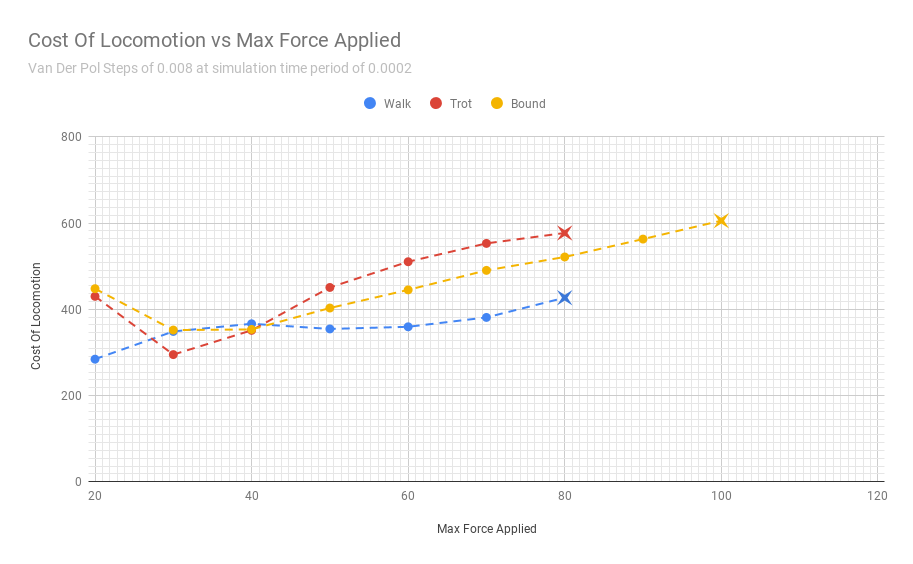
\includegraphics[width=1\textwidth]{figures/fig2.png}
%   \caption{Cost of locomotion per unit distance over force applied.}
%   \label{walktrotbound}
% \end{figure}

% \begin{figure}[h!]
%   \centering
%   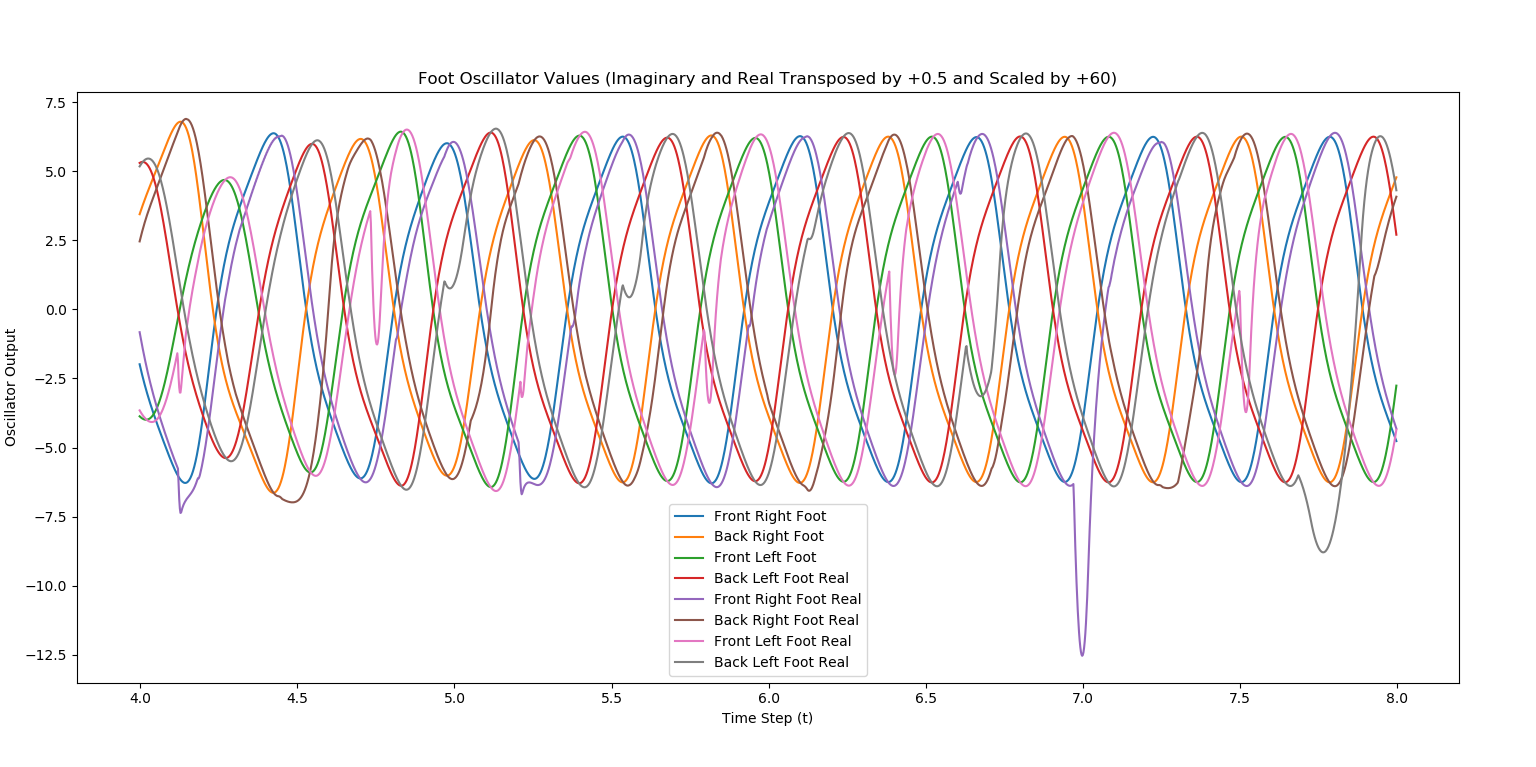
\includegraphics[width=1\textwidth]{USFD_Academic-_Report_LaTeX-Template/figures/oscillatortranspose.png}
%   \caption{Results of reverse transposition and scaling real motor outputs onto oscillator values.}
%   \label{walktrotbound}
% \end{figure}


% \begin{figure}[h!]
%     \centering
%     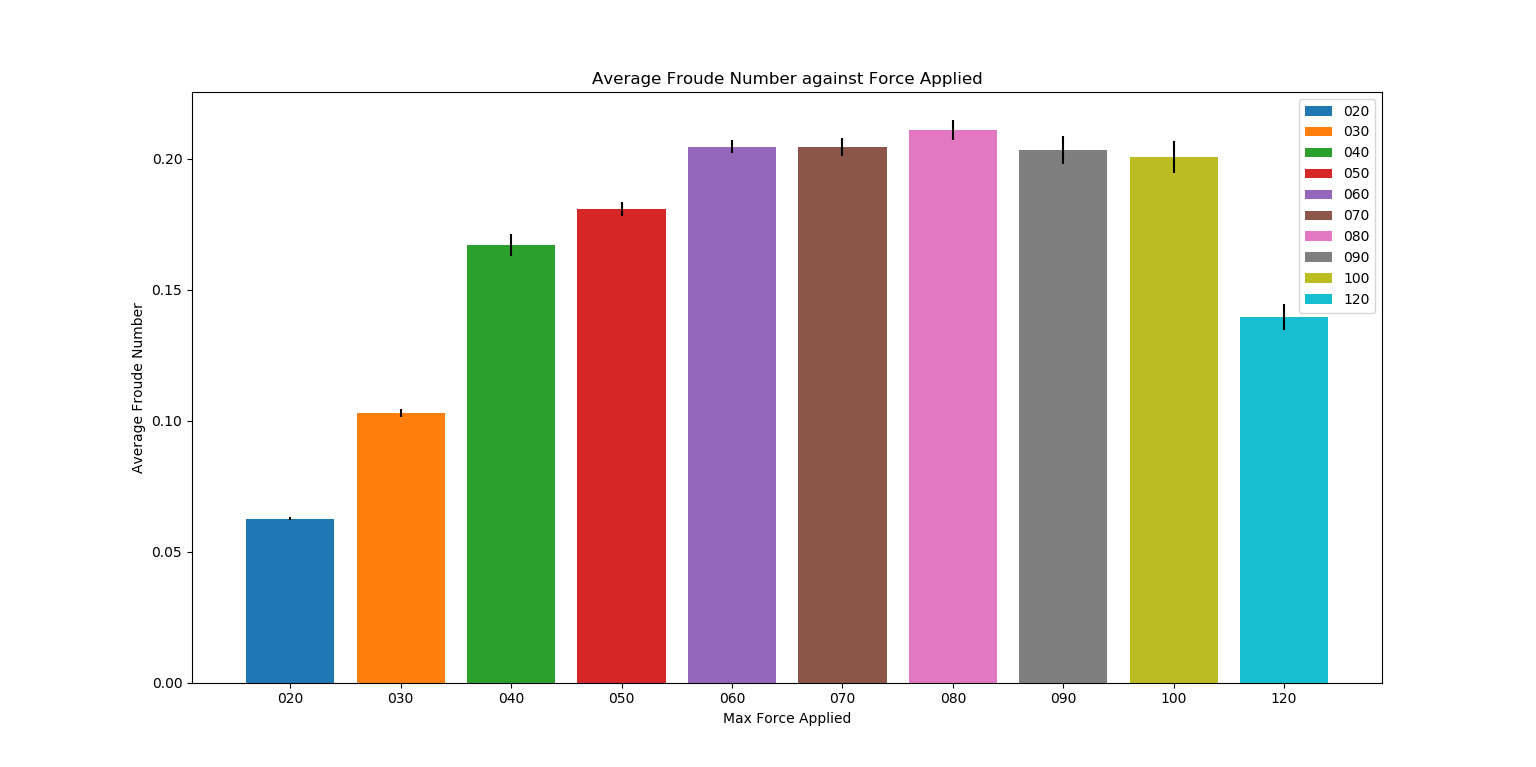
\includegraphics[width=1\textwidth]{USFD_Academic-_Report_LaTeX-Template/figures/froude_number_against_force.png}
%     \label{froudenumbervsforce}
% \end{figure}

% \begin{figure}[h!]
%     \centering
%     \includegraphics[width=1\textwidth]{figures/froudevsforce.png}
%     \caption{Average Froude number against force applied for entire dataset of experiments.}
%     \label{froudenumbervsforce}
% \end{figure}


% \begin{figure}[h!]
%     \centering
%     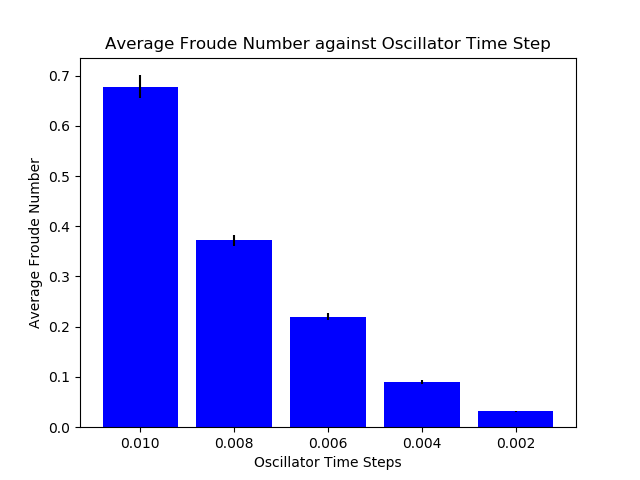
\includegraphics[width=1\textwidth]{figures/froudeosc.png}
%     \caption{Average Froude number against change in oscillator time-step for entire dataset of experiments.}
%     \label{froudenumbervsoscill}
% \end{figure}

% \begin{figure}[h!]
%     \centering
%     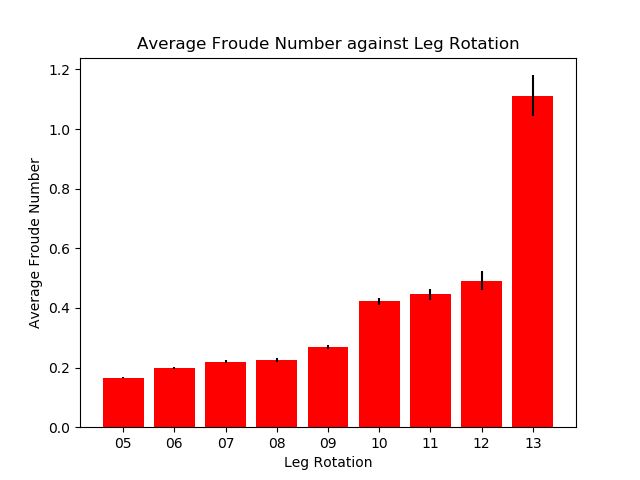
\includegraphics[width=1\textwidth]{figures/froudevsrotation.png}
%     \label{froudenumbervsangle}
%     \caption{Average Froude number against leg rotation for entire dataset of experiments.}
% \end{figure}



% \section{Dynamic Similarity}
% For this paper we will investigate specifically the results seen in relative stride length against froude number, as they are the closest calculation available to be performed. Froude number was investigated against changes in parameter. We focused on the  walking gait in this dissertation due to the large complexity of the system, and the results seen in the initial gait analysis, as even in higher forces, faster gaits still broke down at similar values. This in return can be displayed through a normal graph, as can be seen in 

% \begin{figure}[h!]
%     \centering
%     \includegraphics[width=1\textwidth]{figures/forceandnormal.png}
%     \label{froudenumbervsangle}
% \end{figure}


% Some investigation was done into force values below 20, but we found that this ended with the robot being unable to keep it's own weight. The results of that investigation can be seen in the table in the appendix. 

\section{Discussion}
One of the most interesting results is through the investigation of Froude number values when applying a walking gait. The majority of results for walking gaits, irregardless of oscillator time step, foot angles, or force applied have remained in the regions seen in \cite{Alexander1983}. Namely, Froude numbers below 0.4. As stated in the results, this does mean that almost 30\% of values reach above the limits imposed, however when filtering by oscillator time step, There was an increase the amount of values found in the correct range by (). This shows that the majority of values found above Froude numbers of 0.4 where due to higher oscillator time-steps. These oscillator time-steps may not be attainable realistically as this dissertation did not take into account factors of interlimb friction that may occur in an actual robot/ quadruped mammal. Because of this, it may be that there is a physical limit that does not exist with our robot at faster oscillations. This additionally would suggest that the limiting factor in velocity of a walking gait is the speed the limbs can move at. 

% This can be seen through the following graph. Although there appears to be a steady increase as both oscillator values and rotation angles are increased, this is additionally marked by a high change in variance, making gaits far less stable to changes in force at these values. 



Additionally, maximum gait values in this design are only reaching upwards of 2.0, meaning they remain in the lower bounds of faster gaits. This may be a reason as to why effects of faster gaits have not been successful in this research. This may be due to potential issues with the implementation of our model. This is extremely similar to the results found in \cite{Rutishauser2008}, although the implementation of a Central Pattern Generator is different. This suggests that the implementation of faster gaits such at trots may require additional balancing through the use of real-time feedback. 

Another potential issue which may have skewed the results, and caused faster gaits to be unsuccessful could potentially be caused due to the Laikago model used in the dissertation not having completely accurate mass values. As stated in the implementation stage, although 

% One of the potential reasons as to why many values where found outside of the appropriate bounds of walking may be due to the motors not taking into account real friction that would be seen in animal limbs, although linear damping was set, it may not be fully realistic. The motors themselves where controlled by the velocity control option in PyBullet. 

% As stated in \cite{Alexander1983}, the majority of animals display walking gaits below 0.4. For all of the results in this dissertation, irregardless of force, oscillator time-step or limb rotation, we found that \% of values achieved adhered to this value of froude number.

% Overall, 60.2\% of values where under froude numbers of 0.4, which links towards the same values being found for the majority of animal gaits as seen in \cite{Alexander1983}. The amount of values found above this may be due to the lack of friction against limbs in the environment. This effect is most pronounced on oscillator time-steps of (), where 78\% of values where found to lie under.



% The effects of leg rotation on froude number showcase that there may be a large effects on froude number depending on leg rotation. However, similarly to changes in force, larger changes in leg rotation are met with larger deviations, with stable gaits occuring below a froude number of 0.4. 

% A covariance matrix between cost of locomotion and froude number can be seen below, showcasing how changes in cost of locomotion affect froude number. 

% This seems to coincide with froude number research, and suggests that although our simulated robots can use far faster gaits, there is a higher effect on variation, and as such, walking gaits that use larger angle values may perform faster gaits outside of the range seen in evolutionary circumstances. Although these may be out of range they are essentially symmetric gaits. The reasons as to why a walking gait may still perform well outside of this range is that the 

% Due to the normal distributions seen by the data, as can be seen through






% Distribution was calculated for all experiments ran, with distribution gathered for froude number and cost of locomotion. Froude number distribution can be seen in \ref{froudedistribution} and cost of locomotion distribution can be seen in \ref{costdistribution}. They will be discussed together due to both of them having extremely high continuous distributions with positive skew. Particularly, they both show that there is an extremely large amount of results at, or close to 0 for both froude number and cost of locomotion. This suggests that many of the gaits prove to be unstable and do showcase realistic gait values. Although froude number is shown to be very low in \cite{Alexander1983}, this is still worrying. The following can be seen by filtering the distributions based on force. This showcases the effect that force has on gait value, with variance increasing as force increases. 





% \begin{figure}[h!]
%   \centering
%   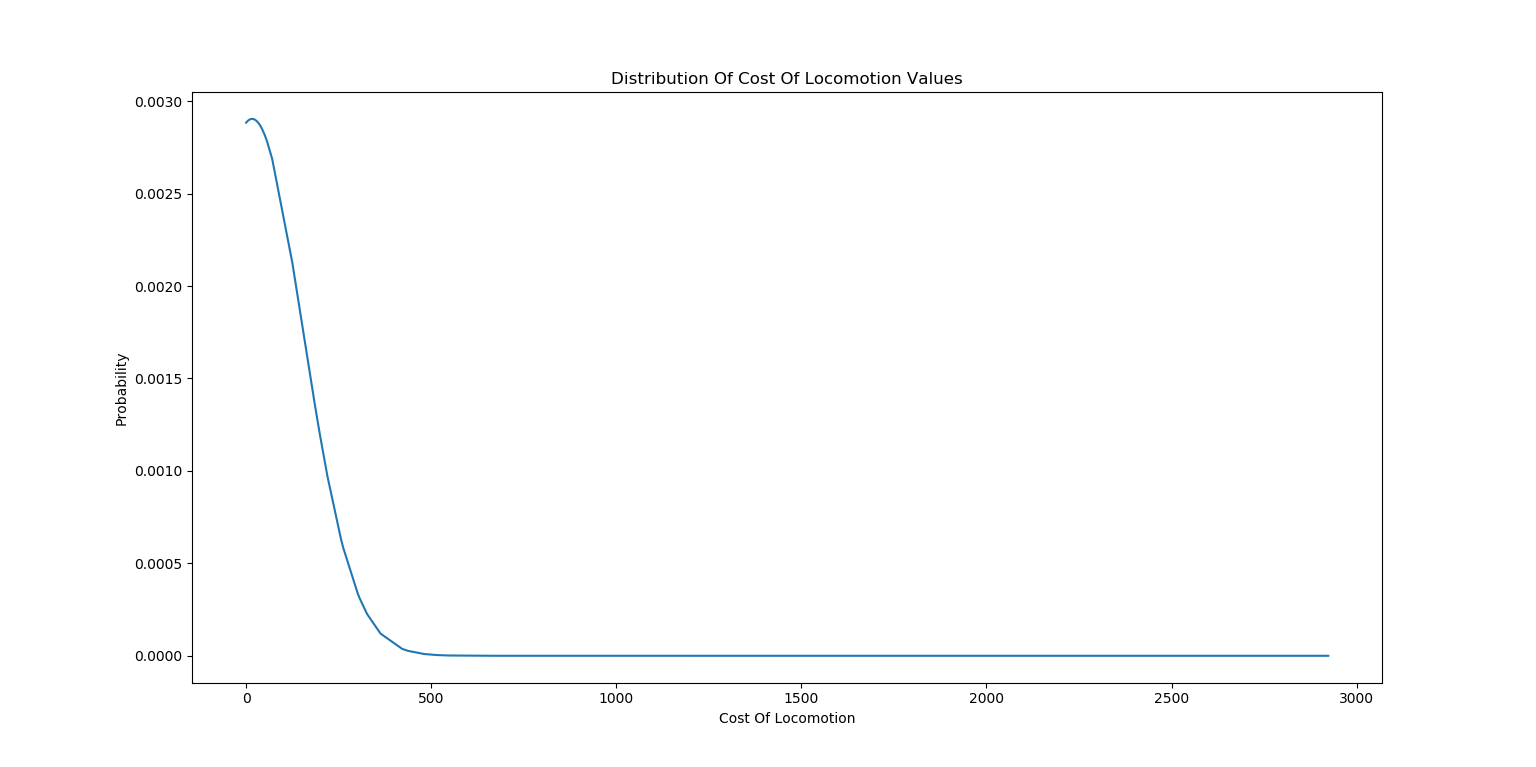
\includegraphics[width=1\textwidth]{USFD_Academic-_Report_LaTeX-Template/figures/costoflocomotiondistribution.png}
%   \caption{Distribution of cost of locomotion per unit distance.}
%   \label{costdistribution}
% \end{figure}

% \begin{figure}[h!]
%   \centering
%   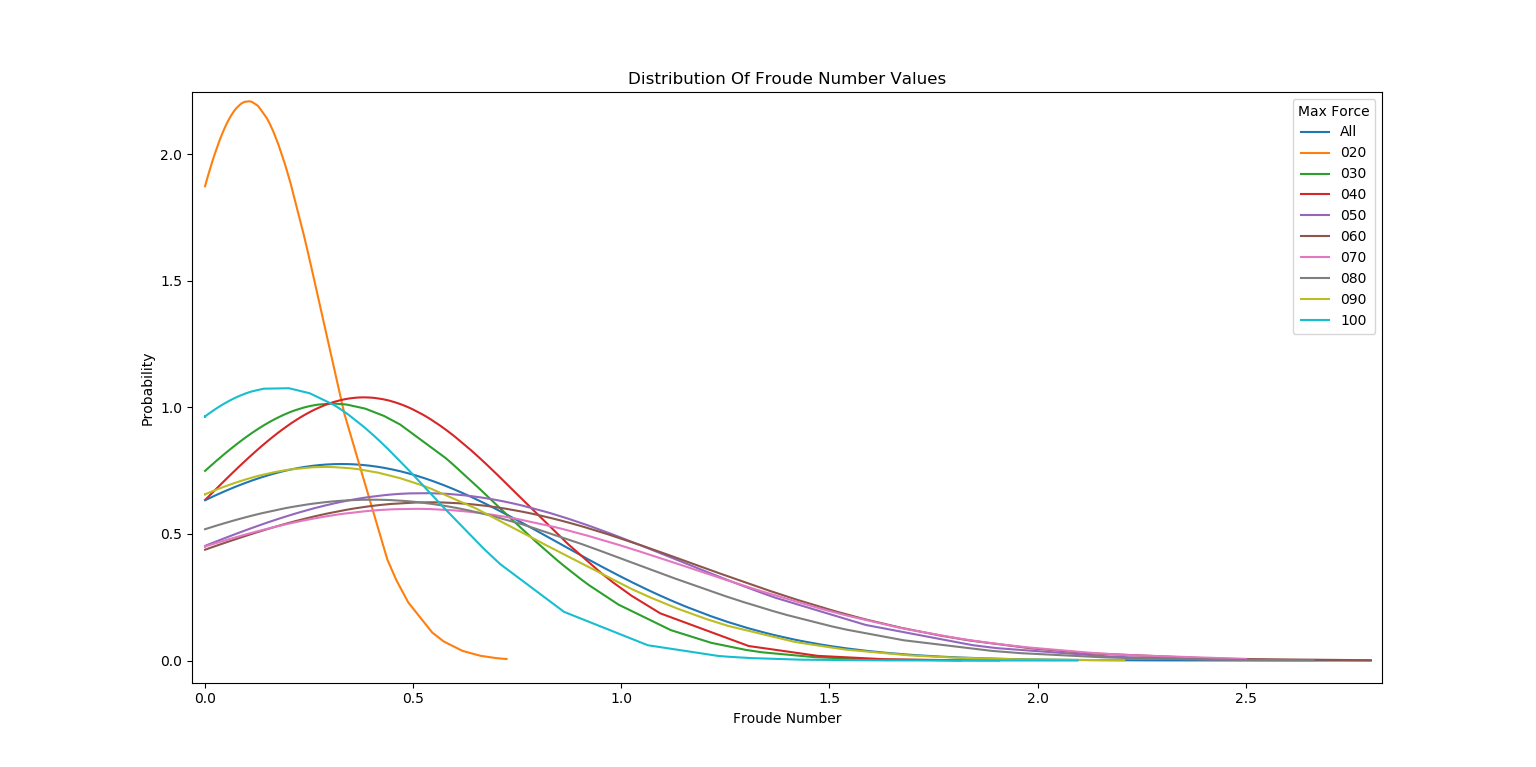
\includegraphics[width=1\textwidth]{USFD_Academic-_Report_LaTeX-Template/figures/froudenforcedistributions.png}
%   \caption{Distribution of cost of locomotion per unit distance.}
%   \label{costdistribution}
% \end{figure}

\section{Further Work}
 Due to the accuracy of pybullet when converting from simulation to real robotics, as seen in \cite{}, further research could be done on comparing the results seen in this work to an actual quadruped robot. As the models seen in this work have been directly based on the Laikago robot, a direct comparison could be made between the experimental results found and actual gait results generated. If a full system identification of the Laikago is made, this could increase the accuracy of the results seen in the paper.

This paper has only dealt with gaits in a limited environment with the test environment confining the animal to travel down a straight line. With the implementation of limb feedback, additional work could be done in effects on the animals CPG through the introduction of obstacles in the environment. More work could potentially be done on the introduction of control into the system, allowing the gaits to change dynamically based on the velocity chosen, as well as a possible implementation of turning through changing coupling.

An interesting, although slightly peculiar potential method for future work is an investigation as to whether the dynamic similarity hypothesis will still hold for different gravity values, as it is part of the equation for Froude Number. This would be an interesting method as it could potentially highlight speeds and gaits that animals should be travelling at in different bodies. For example, if a quadruped robot is attempting to travel on the moon, it would in turn not need to use anything faster than a walking gait, as it would be able to achieve the same velocities without expending as much energy.  

Although out of scope for the project due to time constraints, further work can be done on implementing evolutionary techniques for this project, due to the large amount of free parameters found in this system. This could be done with a similar method as seen in \cite{Geijtenbeek2013}. This could however cause issues with comparisons between Dynamic Similarity, due to faster gaits being possible. A possible solution to this would be investigating different cost functions for robot, such as stability or velocity and comparing them to a cost function related to adhering to Dynamic Similarity. This could show reasons as to why mammals might adhere to the concept of Dynamic Similarity, and provide a new cost function that can be used when designing quadruped mammals.

 Additional work should be done investigating the effectiveness of faster gaits at larger values. One of the main issues with using faster gaits for this project was due to stability, as the robot did not contain any methods of remaining stable when using faster gaits, causing it to fall down when attempting to go quickly. By the implementation of feedback for walking, as well as potential balancing methods as seen in \cite{}, faster gaits, as well as transitions between gaits could be investigated.

After querying the creator of the pybullet engine, it was found that a full system identification had not yet been performed, and as such a 3D model with fully realistic values was not yet implemented in the engine. Once this system identification is complete, there is a potential in re-doing the experiments found in this dissertation, as the full system identification could include more in depth methods such as motor friction.

% Additional work could potentially be done on the application of dynamic similarity to different quadrupeds, through the extension of work done on different models, as the central pattern generator designed in this paper could easily be extended to different robotic models.




